\subsection{Nuggets in Simulation and on Hardware}\label{sec:model_performance_evaluation}

% \begin{figure}[htbp]
%   \centering
%   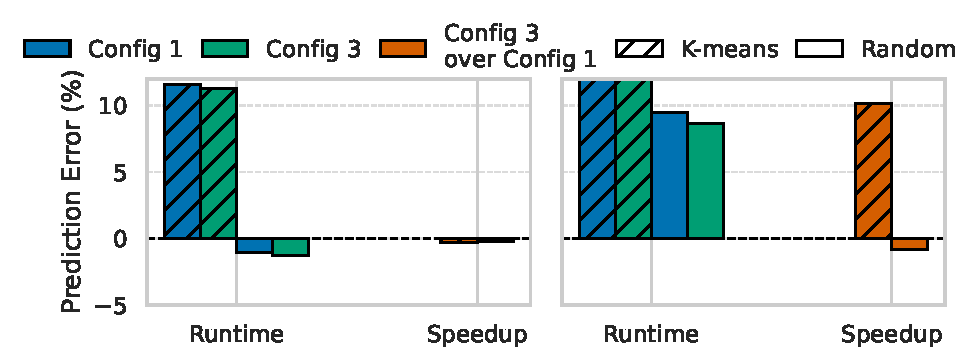
\includegraphics[width=\linewidth]{images/case_study_1_dual.pdf}
%   \caption{Runtime and speedup prediction errors for benchmarks ``cg'' (left) and ``is'' (right) on simulation models.}
%   \label{fig:cg-is-prediction-error}
% \end{figure}

The goal of computer architecture analysis is often to compare the performance of two systems.
Therefore, to investigate the usefulness of nuggets, we run both the entire workload and the nuggets and compare the speedup between different systems.
We compare four different systems \emph{in simulation} to eliminate the potential inaccuracies from the interval selection marker in hardware.
We also compare four different hardware systems.
With these eight systems, we can make two conclusions.
(1) We can use hardware to provide increased confidence in the selected intervals, but we cannot prove or bound the error due to the overheads discussed in Section~\ref{sec:case_study_simulation_results}.
(2) We find that Random and basic-block vector approaches to interval selection are not microarchitectural independent.
In fact, we find that microarchitectural differences affect the accuracy of the selection methodology more than the ISA.

% To demonstrate that hardware can be used to validate the effectiveness of the sample set in evaluating simulation models with different ISAs and microarchitectures, we show how nuggets executed on real hardware can provide insight into the variance of the prediction error and help build confidence in the selected samples.
% We then use simulation data to analyze the factors that most influence prediction error using three case studies.
% The key take aways are that 1) \textbf{validating samples on real hardware is more efficient than simulation and provides a reliable understanding of prediction error variability}, and 2) \textbf{microarchitectural differences impact program phases more significantly than architectural (ISA) differences}.

% We use speedup prediction error as our primary metric because our experimental results show that large runtime prediction errors do not necessarily translate to large speedup prediction errors, which speedup is the more relevant metric in system evaluation.
% % For example, in Figure~\ref{fig:cg-is-prediction-error}, the ``cg'' benchmark shows that both K-means and Random selected samples achieve near zero speedup prediction error, despite exhibiting runtime prediction errors of 11\% (K-means) and -1\% (Random) for the two simulation models.
% For example, the ``cg'' benchmark shows that both K-means and Random selected samples achieve near zero speedup prediction error, despite exhibiting runtime prediction errors of 11\% (K-means) and -1\% (Random) for the two simulation models.
% A similar trend is observed for the ``is'' benchmark.
% Even when runtime errors exceed 100\%, as seen with ``is'' using K-means-selected nuggets, the resulting speedup predictions can remain accurate (within 5\%), indicating that speedup is more resilient to absolute runtime fluctuations.
% Therefore, we focus on the \emph{consistency} of relative errors across configurations rather than on absolute runtime prediction errors.

In this thesis we report the \emph{error in predicted speedup}, not the error in absolute runtime.
We found that in cases with modest absolute error the predicted speedup (or relative performance) is often much more accurate.

% We use speedup prediction error as our primary metric because large runtime errors do not necessarily translate to large speedup prediction errors.
% For example, in the ``cg'' benchmark, both K-means and Random samples achieve speedup prediction errors within 2\% in Config~3 over Config~4, despite runtime errors of 11\% and $-1\%$, respectively.
% Similarly, for ``is'', K-means-selected nuggets show over 100\% runtime error but maintain a speedup prediction error within 1\% for Config~3 over Config~4.
% We argue that speedup is more important because performance can only be evaluated through comparison.
% Therefore, we focus on the \emph{consistency} of relative errors across configurations rather than on absolute runtime prediction errors.

\subsubsection{Experimental Setup}

\begin{table}[!t]
  \centering
  \scriptsize  % smaller than \small
  \setlength{\tabcolsep}{3pt}
  \renewcommand{\arraystretch}{1.2}

  \begin{tabular}{|c|c|c|c|c|}
    \hline
    \textbf{Model}
      & \textbf{ISA}
      & \textbf{Core}
      & \textbf{Cache Hierarchy}
      & \textbf{Memory} \\ \hline

    Config 1
      & x86
      & \makecell[l]{4-core Large OOO\\@ 4~GHz}
      & \makecell[l]{L1d: 64~KiB L1i: 64~KiB\\L2: 1~MiB}
      & \makecell[l]{DDR4 2400~MHz\\38.4~GB/s} \\ \hline

    Config 2
      & Arm
      & \makecell[l]{8-core Small OOO\\N1 @ 3~GHz}
      & \makecell[l]{L1d: 64~KiB L1i: 64~KiB\\L2: 1~MiB SLC: 32~MiB}
      & \makecell[l]{DDR4 2400~MHz\\76.8~GiB/s} \\ \hline

    Config 3
      & x86
      & \makecell[l]{4-core Base OOO\\@ 4~GHz}
      & \makecell[l]{L1d: 64~KiB L1i: 64~KiB\\L2: 1~MiB}
      & \makecell[l]{DDR4 2400~MHz\\38.4~GB/s} \\ \hline

    Config 4
      & Arm
      & \makecell[l]{8-core Base OOO\\@ 4~GHz}
      & \makecell[l]{L1d: 64~KiB L1i: 64~KiB\\L2: 1~MiB}
      & \makecell[l]{DDR4 2400~MHz\\76.8~GiB/s} \\ \hline

  \end{tabular}

  \caption{gem5 Simulation Model Configuration. \revision{The large, small, and base out-of-order cores are internal models that target different performance characteristics.}}
  \label{tab:system-configuration-simulation}
\end{table}


We use the selected nuggets to conduct experiments on both gem5, using full-system simulation, and real hardware.
In addition to the systems listed in Table~\ref{tab:system-configuration}, we include two additional real hardware platforms: an Intel i9-9900X system and an Intel i7-9700 system.
The simulation models used are listed in Table~\ref{tab:system-configuration-simulation} and run a guest Ubuntu~24.04 kernel, matching the software environment of the real hardware.

Sample sets are selected using the ``Random'' and ``K-means'' methods described in Section~\ref{sec:sampling_methodology}.
We set $k = 20$ in this experiment, as the use of NPB Class A with a single-threaded configuration results in a relatively small pool of intervals available for sampling.
Single-threaded workloads also help eliminate confounding factors such as thread interleaving, which could otherwise affect our measurement of prediction error.

% The selected nuggets are executed on both the gem5 simulator and real hardware, with runtime measured for each nugget.
% We also execute the full workload on both real hardware and simulation models to obtain baseline runtimes.

In simulation, we use gem5 to track sample interval markers directly, thereby avoiding the runtime overhead introduced by hook-based marking mechanisms.
To simulate nuggets efficiently, we first use KVM to fast-forward execution to the warmup marker and then create a gem5 checkpoint~\cite{gem5-checkpoints}.
This allows us to resume nugget execution from that point using different microarchitectural configurations, subject to certain constraints (e.g., the number of cores must remain fixed).
For each nugget, we restore from the checkpoint and begin measurement only after reaching the start marker, allowing the microarchitectural state to warm up naturally.

\subsubsection{Results}\label{sec:case_study_simulation_results}

\paragraph*{Hardware-Based Validation Offers Scalability and Early Signal}

Validating samples on real hardware is significantly faster and more scalable than using simulation.
Several simulation runs (e.g., ``bt'', ``lu'', and ``sp''), even with small inputs such as Class A, remain incomplete after two weeks, making simulation impractical for extensive validation.
By contrast, hardware validation enables us to quickly assess the variability in speedup prediction across platforms.
% If the prediction error remains consistent across diverse systems, it suggests that the selected samples are representative and robust for the prediction task.

% \begin{figure}[htbp]
%   \centering
%   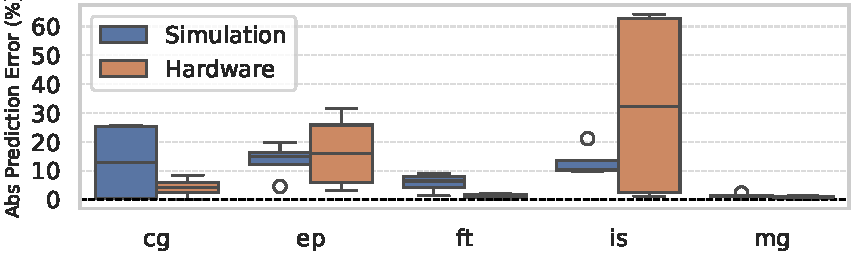
\includegraphics[width=\linewidth]{images/case_study_2.pdf}
%   \caption{Distribution of absolute speedup prediction errors using K-means samples across simulation (blue) and hardware (orange) comparisons for selected benchmarks. Hardware-based comparisons provide early indications of variability in prediction accuracy.}
%   \label{fig:abs-speedup-prediction-error-var}
% \end{figure}

\begin{figure}[!t]
  \centering
  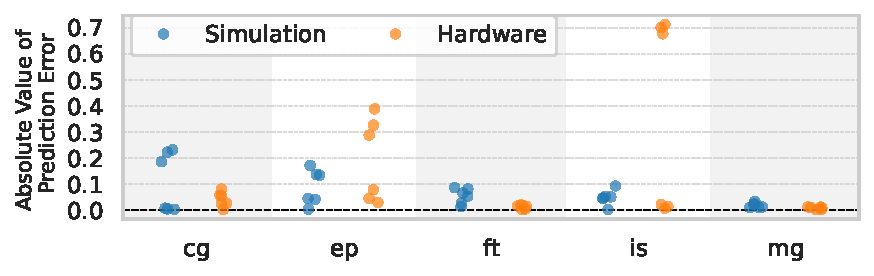
\includegraphics[width=\linewidth]{images/case_study_2_jitter.pdf}
  \caption{Distribution of absolute speedup prediction errors using K-means samples across simulation (blue) and hardware (orange) comparisons for selected benchmarks. ``0.1'' means 10\% difference in predicted speedup.}
  \label{fig:abs-speedup-prediction-error-var}
\end{figure}

Figure~\ref{fig:abs-speedup-prediction-error-var} shows the distribution of absolute speedup prediction errors for selected benchmarks.
Each point is absolute value of the error of one pair of configurations' (in simulation) or pair of hardware systems' speedup compared to the true speedup of those two systems determined by running the entire workload.
% We focus on absolute error because the direction of the prediction error can vary depending on the system pair being compared, and our goal is to capture the magnitude of error regardless of direction.
The hardware results allow us to quickly identify benchmarks with high variability in prediction error, such as ``cg'', ``ep'', and ``is'', which exhibit wide error ranges across different platforms.
For these workloads with large variations or large errors on hardware, we find the intervals are \emph{not representative of the true speedup}.
However, we cannot use the error on hardware to bound the error in simulation (e.g., the error for ft in simulation is larger than on hardware).
The main reason we cannot use the hardware error to bound the simulation error is that the error is strongly affected by the underlying microarchitecture.
% We observe a broader distribution of prediction errors in hardware because the real systems used exhibit greater microarchitectural diversity than the simulation models we use for this experiment.
In the next section, we analyze the sources of prediction error in more detail using simulation data and controlled case studies.

\paragraph*{ISA vs. Microarchitecture: Case Study}

To isolate the sources of prediction error, we compare three types of platform pairs:
(1) systems with different ISAs but small \revision{microarchitecture} differences,
(2) systems with significantly different microarchitectural configurations, but the same ISA, and
(3) systems that differ in both ISA and microarchitecture.

\begin{figure}[!t]
  \centering

  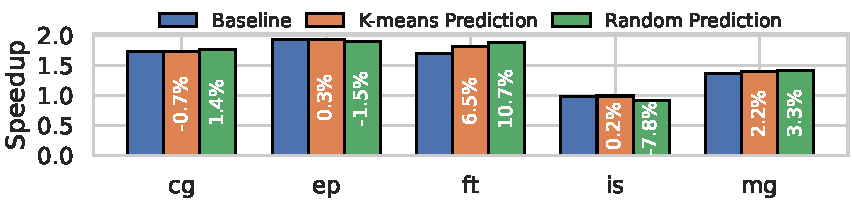
\includegraphics[width=\linewidth]{images/case_study_3.pdf}
  \caption{Speedup: Random vs.\ K-means samples when ISA varies and microarchitecture is fixed, Config~3 vs.\ Config~4.}
  \label{fig:case_study_3}
\end{figure}

Figure~\ref{fig:case_study_3} shows the speedup prediction error when the main difference between platforms is the ISA (Config~3 vs.\ Config~4).
% These configurations share similar microarchitectures but differ in ISA (x86 vs. Arm).
In this experiment, the ISA has a noticeable impact on the binaries: for instance, the Arm binaries have vectorization enabled, whereas the x86 binary does not.
The average absolute speedup prediction error is 5\% for Random-selected nuggets and 2.0\% for K-means-selected nuggets.
Among all benchmarks, ``ft'' exhibits the highest K-means error (6.5\%), likely due to an unrepresentative sample set.
A linear regression of nugget runtimes across the two ISAs explains 94.5\% of the variance, indicating that the selected samples capture similar execution phases across architectures.
The K-means speedup error for ``ft'' is consistent with its runtime prediction errors on Config~3 (4.9\%) and Config~4 (--1.5\%), suggesting the overestimation stems from sample imbalance.
This implies that certain performance-critical phases were not captured by the selected nuggets.
The Random-selected samples show a similar pattern for both the ``ft'' and ``is''.

\begin{figure}[!t]
  \centering
  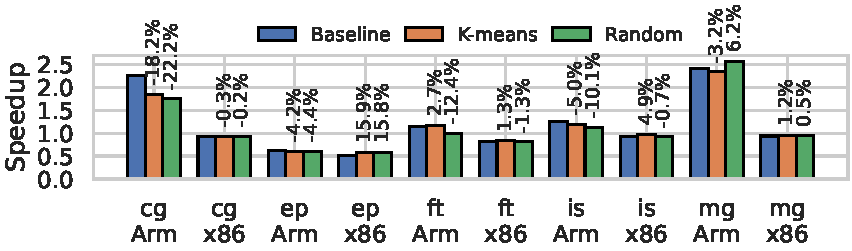
\includegraphics[width=\linewidth]{images/case_study_4.pdf}
  \caption{Speedup between Random and K-means samples when microarchitecture varies and ISA is fixed: Config~4 over Config~2 for Arm, and Config~3 over Config~1 for x86.}
  \label{fig:case_study_4}
\end{figure}

Figure~\ref{fig:case_study_4} shows the speedup prediction error when the microarchitecture varies: Config~4 over Config~2 for Arm and Config~3 over Config~1 for x86.
The average absolute prediction error increases to 8.1\% for Random-selected nuggets and 5.9\% for K-means-selected nuggets.
The comparison between Config~4 and Config~2 for Arm results in higher error in predicted speedup using the selected nuggets than between Config~3 and Config~1 for x86, reflecting greater microarchitectural differences in the Arm systems despite running the same benchmarks and sample sets.

\begin{figure}[!t]
  \centering
  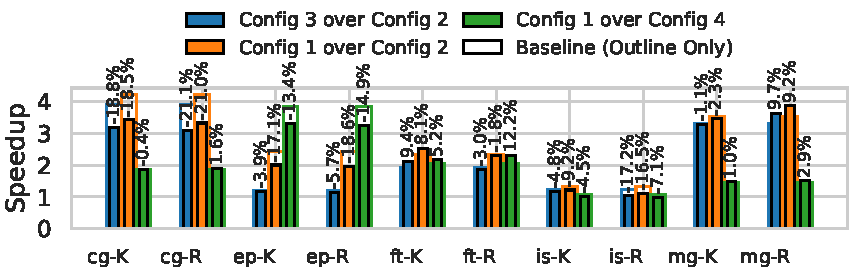
\includegraphics[width=\linewidth]{images/case_study_5.pdf}
  \caption{Speedup comparison between Random and K-means samples when both ISA and microarchitecture vary across simulation models.
  ``K'' indicates K-means samples, and ``R'' indicates Random samples.}
  \label{fig:case_study_5}
\end{figure}

Figure~\ref{fig:case_study_5} presents the speedup prediction error when both ISA and microarchitecture vary across simulation models.
The average absolute error rises to 10.8\% for Random-selected nuggets and 7.9\% for K-means-selected nuggets.
The lowest errors occur in comparisons between Config~1 and Config~4 (7.7\% for Random, 5\% for K-means), where microarchitectural differences are relatively minor.
In contrast, we observe larger errors in comparisons involving Config~2, which diverges significantly from other configurations in both ISA and microarchitecture.
These findings highlight the sensitivity of prediction accuracy to microarchitectural differences more than to ISA variation.

\textbf{In summary}, while this thesis does not propose a new method for selecting representative intervals, we show the importance of comparing different interval selection techniques across a wide variety of architectures and microarchitectures.
Nugget enables future work to have apples-to-apples comparisons across architectures and fast comparisons on hardware opening this new line of research.

% \textbf{In summary}, the case studies reveal that ISA differences have minimal impact on speedup prediction accuracy, whereas microarchitectural variations contribute more significantly to prediction error.
% This motivates us to validate the selected samples using a range of microarchitectural configurations, as these are more likely to influence the execution phases captured by the samples.
% Using real hardware enables faster validation and provides broader coverage of microarchitectural diversity.
% Additionally, the K-means sampling strategy—based on LLVM IR basic block (IRBB) vectors—consistently yields more accurate speedup predictions across all configurations compared to the Random strategy, while requiring fewer samples on average.
% Specifically, Random consistently selects 20 nuggets per benchmark, whereas K-means selects an average of 13 (range: 2--20), achieving better accuracy with lower sampling overhead.
